\documentclass{article}

\usepackage[utf8]{inputenc}
\usepackage[english]{babel}
\usepackage[%
    left=1.30in,%
    right=1.30in,%
    top=1.0in,%
    bottom=1.0in,%
]{geometry}%
\usepackage{float}
\usepackage{amsfonts}
\usepackage{mathtools}
\usepackage{graphicx}
\usepackage{csquotes}
\usepackage{biblatex}
\usepackage{tikz}
\usepackage[colorlinks=true]{hyperref}

\addbibresource{bibliography.bib}
\graphicspath{ {./images/} }

\newcommand{\defeq}{
    \stackrel{def}{=}
}
\newcommand{\tablegraphics}[2]{
    \raisebox{-.5\height}{\includegraphics[scale=#2]{#1}}
}
\DeclarePairedDelimiter{\norm}{\lVert}{\rVert}
\usetikzlibrary{positioning,arrows.meta,calc,fit}
\def\trapW{3}
\def\trapHa{.9}
\def\trapHb{2}
\def\borderW{0.2mm}
\def\imgscl{.7}
\def\lrgimgscl{.5}

\newcommand{\recfigfragment}[7]{
    \textbf{#1} & \tablegraphics{#2/#3}{\imgscl} & \tablegraphics{#2/#4}{\imgscl} & \tablegraphics{#2/#5}{\imgscl} & \tablegraphics{#2/#6}{\imgscl} & \tablegraphics{#2/#7}{\imgscl}
}

\newcommand{\recfig}[5]{
    \begin{figure}[H]
    \centering
    \bgroup
    \def\arraystretch{4}
    \begin{tabular}{c c c c c c}
    \hline\hline
    \recfigfragment{Original images}{frogs}{frog-#1}{frog-#2}{frog-#3}{frog-#4}{frog-#5} \\
    \hline
    \recfigfragment{GLO}{glototalrec}{#1-fake}{#2-fake}{#3-fake}{#4-fake}{#5-fake} \\
    \hline
    \recfigfragment{Our (without term)}{ournopertrec}{#1-fake}{#2-fake}{#3-fake}{#4-fake}{#5-fake} \\
    \hline
    \recfigfragment{Our (with term)}{ourrec}{#1-fake}{#2-fake}{#3-fake}{#4-fake}{#5-fake} \\
    \hline\hline
    \end{tabular}
    \setlength{\tabcolsep}{5em}
    \egroup
    \caption{A few reconstructions of training images}
    \end{figure}
}

\newcommand{\encrecfig}[6]{
    \begin{figure}[H]
    \centering
    \bgroup
    \def\arraystretch{4}
    \begin{tabular}{c c c c c c}
    \hline\hline
    \recfigfragment{Original images}{frogs}{frog-#1}{frog-#2}{frog-#3}{frog-#4}{frog-#5} \\
    \hline
    \recfigfragment{Reconstructed}{encrec}{#1-fake}{#2-fake}{#3-fake}{#4-fake}{#5-fake} \\
    \hline\hline
    \end{tabular}
    \setlength{\tabcolsep}{5em}
    \egroup
    \caption{A few reconstructions of #6 images}
    \end{figure}
}

\newcommand{\interfig}[4]{
    \begin{figure}[H]
    \centering
    \bgroup
    \def\arraystretch{5}
    \begin{tabular}{c c}
    \hline\hline
    \textbf{GLO} & \tablegraphics{glototalinter/#1-#2n}{\lrgimgscl} \\
    \hline
    \textbf{Our (without term)} & \tablegraphics{ournopertinter/#1-#2n}{\lrgimgscl} \\
    \hline
    \textbf{Our (with term)} & \tablegraphics{ourinter/#1-#2n}{\lrgimgscl} \\
    \hline\hline
    \end{tabular}
    \setlength{\tabcolsep}{5em}
    \egroup
    \caption{An interpolation of #4 images (#3)}
    \end{figure}
}
\tikzset
{
  Trapezium/.pic =
  {
    \draw [line width=\borderW] (0,0) -- (0,\trapHa) -- (\trapW,\trapHb) -- (\trapW,-\trapHb) -- (0,-\trapHa) -- cycle ;
    \coordinate (-center) at (\trapW/2,0);
    \coordinate (-out) at (\trapW,0);
  },
  Arrow/.style=
  {
    line width=2mm,
    -{Triangle[length=2.5mm,width=5mm]},
    shorten >=2pt,
    shorten <=2pt,
  }
}
\newcommand{\EncoderDecoder}{
\begin{figure}[H]
\centering
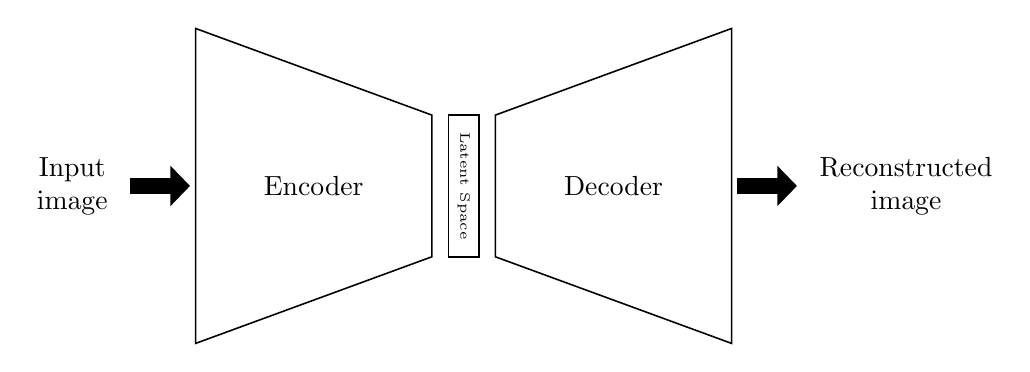
\begin{tikzpicture}
[
  node distance=2mm, % space between drawn parts
  every node/.style={align=center},
]
\node (latSpace) 
  [
    draw,
    line width=\borderW,
    minimum height=2*\trapHa cm,
    font=\tiny,
  ]
  {\rotatebox{-90}{Latent Space}};
  \pic (left)[left=of latSpace.west, rotate=180] {Trapezium};
  \pic (right)[right=of latSpace.east] {Trapezium};
  \node at (left-center) {Encoder};
  \node at (right-center) {Decoder};
  
  \def\d{.9}
  \coordinate (u) at (\d,0);
  \draw [Arrow] (right-out) -- ++(u) node [anchor=west] {Reconstructed\\image};
  \draw [Arrow] ($(left-out)-(u)$) node [anchor=east] {Input\\image} -- ++(u) ;
\end{tikzpicture}
\caption{Illustration of the architecture}
\end{figure}
}